\documentclass[UTF8]{article}
\usepackage{listings}
\usepackage{xcolor} %颜色
\usepackage{graphicx}%插入图片
\usepackage{booktabs} %绘制表格
\usepackage{caption2} %标题居中
\usepackage{geometry}
\usepackage{array}
\usepackage{amsmath}
\usepackage{subfigure} 
\usepackage{longtable}%表格
\usepackage{abstract}
\usepackage{appendix}%附录
\usepackage{ctex}
\setCJKfamilyfont{adobesong}{Adobe Song Std}
\pagestyle{plain} %页眉消失
\setlength{\parindent}{0pt}
\usepackage{indentfirst} % 首行缩进
\setlength{\parindent}{2em}
\geometry{a4paper,left=2.5cm,right=2.5cm,top=2.5cm,bottom=2.5cm}
\definecolor{mygreen}{rgb}{0,0.6,0}
\definecolor{mygray}{rgb}{0.5,0.5,0.5}
\definecolor{mymauve}{rgb}{0.58,0,0.82}
\lstset{ %
backgroundcolor=\color{white},   % choose the background color
basicstyle=\footnotesize\ttfamily,        % size of fonts used for the code
columns=fullflexible,
breaklines=true,                 % automatic line breaking only at whitespace
captionpos=b,                    % sets the caption-position to bottom
tabsize=4,
commentstyle=\color{mygreen},    % comment style
escapeinside={\%*}{*)},          % if you want to add LaTeX within your code
keywordstyle=\color{blue},       % keyword style
stringstyle=\color{mymauve}\ttfamily,     % string literal style
frame=single,
rulesepcolor=\color{red!20!green!20!blue!20},
% identifierstyle=\color{red},
language=c++,
}

\lstset{
		numbers=left, %设置行号位置
		numberstyle=\tiny, %设置行号大小
		keywordstyle=\color{blue}, %设置关键字颜色
		commentstyle=\color[cmyk]{1,0,1,0}, %设置注释颜色
		escapeinside=``, %逃逸字符(1左面的键)，用于显示中文
		breaklines, %自动折行
		extendedchars=false, %解决代码跨页时，章节标题，页眉等汉字不显示的问题
		xleftmargin=1em,xrightmargin=1em, aboveskip=1em, %设置边距
		tabsize=4, %设置tab空格数
		showspaces=false %不显示空格
	}

\title{Notes About Upgrade II Software }
\author{傅逸\lower-1.0ex\hbox{\scalebox{1}[0.4]{日}}\lower.1ex\hbox{\kern-1em \scalebox{1}[0.5]{升}}}



\begin{document}
    \maketitle
	\newpage

\section{背景介绍}

\subsection{放疗进行肿瘤治疗的原理}

放射治疗是一种利用各种射线（如高能X射线、$\gamma$射线、$\beta$射线、高能电子束、质子、重离子等）产生的电离辐射对疾病（主要是恶性肿瘤）进行治疗的临床手段。

近年来，随着计算机技术、影像诊断、医学物理及生物学的快速发展，恶性肿瘤治疗逐步迈入精准医学时代。围绕临床需求，各学科正致力于推动低毒高效的精准肿瘤放疗技术创新，使放疗在肿瘤治疗中占据了举足轻重的地位。
\subsection{探测器模拟在研究放疗中的作用}
Geant4 通过蒙特卡罗（Monte Carlo, MC）方法精确模拟辐射与物质的相互作用，为放疗的 剂量计算、治疗计划优化、设备设计等提供关键数据支持。Geant4 可以模拟不同粒子（光子、电子、质子、重离子等）在人体组织中的能量沉积，生成高精度的三维沉积能量分布图，帮助评估肿瘤靶区的辐射覆盖和周围正常组织的保护。
\subsection{BCNT 硼中子俘获疗法介绍}
BNCT的基本原理是将含$^{10}$B药物注入患者体内~\cite{WOS:000366954100038}，含$^{10}$B药物靶向性地聚集于肿瘤细胞内后，使用热中子束对病人进行照射，中子被$^{10}$B俘获发生$^{10}$B$(n, \alpha)^{7}$Li反应产生0.478~MeV瞬发$\gamma$射线（93.7\%）,或是直接沉积2.89~MeV能量（6.3\%）。

\section{Geant 4模拟代码}
\subsection{利用Genat 4构建探测器}
此章节既介绍我们的DetectorConstruction。

首先是构造探测器的几何，在这部分我们定义了world、人体（非肿瘤区域），肿瘤区域的几何体积的相关参数，为了展示简洁，具体代码参数设定省去。
\begin{lstlisting}
// World set
    auto worldSizeXY = 1.*m;//定义world的体积
    auto worldSizeZ  = 2.5 * m;//注意粒子枪的位置需不需要在world里?

    // HEAD set
    double head_r = 90 * mm;
    double z_offset = 5*cm;
    double head_pos_x = 0;
    double head_pos_y = 0;
    double head_pos_z = (25 + 9 + 9) * cm - z_offset;
    // Body set
    ...
    // LEG set
    ...
    // Tissue set
    ...
    // Neck set
    ...
\end{lstlisting}
\newpage
接下来，我们定义了材料
\begin{lstlisting}
    G4NistManager* nist = G4NistManager::Instance();

    auto worldMaterial = nist->FindOrBuildMaterial("G4_AIR");//定义G4Material的对象
    auto tissueMaterial = nist->FindOrBuildMaterial("G4_TISSUE_SOFT_ICRP"); // Can also be G4_WATER

    // 各组分的材料密度（需要精确值）
    const G4double tissueDensity = tissueMaterial -> GetDensity();
    const G4double densityB10 = 2.37 * g / cm3;     // 纯B-10密度（需根-据实际形态调整）, set it to be tissueDensity if assume the density unchanges.

    //Boron concentration (ppm)
    const G4double NormalBoronMassFraction = 6 * mg / kg;    // ppm
    const G4double tumorBoronMassFraction = 30 * mg / kg;    // 30 ppm, varies within (30, 200). //must recompile each time it was changed.

    // 创建纯B-10同位素元素
    G4double B10MoleMass = 10.0129370 * g / mole;
    G4Isotope* isoB10 = new G4Isotope("B10", 5, 10, B10MoleMass);
    G4Element* elB10 = new G4Element("EnrichedBoron", "B10", 1);
    elB10->AddIsotope(isoB10, 100.00*perCent);

    //Tumor tissue----------------------
      
      const G4double tumorTissueMassFraction = 1.0 - tumorBoronMassFraction;

      // 计算混合密度（质量加权倒数法）
      G4double invDensityMix = 
          (tumorTissueMassFraction / tissueDensity) + 
          (tumorBoronMassFraction / densityB10);
      G4double TumorDensityMix = 1.0 / invDensityMix;  // 混合后密度

      // 创建材料（按质量分数添加）
      G4Material* TumorTissue = new G4Material(
          "BoronDopedTissue",
          TumorDensityMix,           // 计算得到的混合密度
          2,                    // 
          kStateLiquid,         // 液态
          (36.5+273.15)*kelvin  // 温度
      );
      TumorTissue -> AddMaterial(tissueMaterial, tumorTissueMassFraction);
      TumorTissue->AddElement(elB10, tumorBoronMassFraction);

    //Normal tissue-----------------------
      
      const G4double NormalTissueMassFraction = 1.0 - NormalBoronMassFraction;
      
      // 计算混合密度（质量加权倒数法）
      invDensityMix = 
          (NormalTissueMassFraction / tissueDensity) + 
          (NormalBoronMassFraction / densityB10);
      G4double NormalDensityMix = 1.0 / invDensityMix;  // 混合后密度

      // 创建材料（按质量分数添加）
      G4Material* NormalTissue = new G4Material(
          "BoronDopedTissue",
          NormalDensityMix,           // 计算得到的混合密度
          2,                    // 
          kStateLiquid,         // 液态
          (36.5+273.15)*kelvin  // 温度
      );
      NormalTissue -> AddMaterial(tissueMaterial, NormalTissueMassFraction);
      NormalTissue->AddElement(elB10, NormalBoronMassFraction);
    
\end{lstlisting}

接下来逐行讲解我们的代码

首先是初始化 NIST 材料管理器：
\begin{lstlisting}
    G4NistManager* nist = G4NistManager::Instance();
\end{lstlisting}
获取 Geant4 内置的NIST 材料数据库管理器，用于调用预定义标准材料。
接下里我们定义基础材料：
\begin{lstlisting}
    auto worldMaterial = nist->FindOrBuildMaterial("G4_AIR");
    auto tissueMaterial = nist->FindOrBuildMaterial("G4_TISSUE_SOFT_ICRP");
\end{lstlisting}
其中
\begin{itemize}
    \item \texttt{G4\_AIR}: 模拟环境（如治疗室）的默认材料，材料是使用的空气。
    \item \texttt{G4\_TISSUE\_SOFT\_ICRP}: ICRP 定义的标准化软生物组织，用来模拟受治疗者的身体材料。
\end{itemize}
然后为了模拟使用硼靶向药物后的肿瘤，我们还进行了材料参数设置。
首先进行密度定义
\begin{lstlisting}
const G4double tissueDensity = tissueMaterial->GetDensity();
const G4double densityB10 = 2.37 * g / cm3;    
\end{lstlisting}
\begin{itemize}
    \item \texttt{tissueDensity}: 软组织密度（约 $1.0\,\text{g/cm}^3$）
    \item \texttt{densityB10}: 硼-10同位素密度
\end{itemize}
然后是硼浓度（ppm）定义，根据我们查找的论文，BCNT所使用的靶向药物的硼浓度一般为$10^2$ppm的量级~\cite{ WOS:000427513100016}
\begin{lstlisting}
const G4double NormalBoronMassFraction = 6 * mg / kg;
const G4double tumorBoronMassFraction = 30 * mg / kg;  
\end{lstlisting}
这里则是BNCT关键参数：肿瘤组织需富集更高浓度硼-10（通常为正常组织的5-10倍）。
接下来创建硼-10同位素元素
\begin{lstlisting}
G4double B10MoleMass = 10.0129370 * g / mole;
G4Isotope* isoB10 = new G4Isotope("B10", 5, 10, B10MoleMass);
G4Element* elB10 = new G4Element("EnrichedBoron", "B10", 1);
elB10->AddIsotope(isoB10, 100.00*perCent);    
\end{lstlisting}
其中
\begin{itemize}
    \item \texttt{G4Isotope}: 定义硼-10原子核（质子数=5，中子数=10）
    \item \texttt{G4Element}: 创建纯硼-10元素（摩尔质量$\approx10.013\,\text{g/mol}$）
\end{itemize}
在定义完前面提到的材料后，则可以构建掺杂硼的组织材料了。
对于肿瘤组织（高硼浓度）
\begin{lstlisting}
G4Material* TumorTissue = new G4Material("BoronDopedTissue", ...);
TumorTissue->AddMaterial(tissueMaterial, tumorTissueMassFraction);
TumorTissue->AddElement(elB10, tumorBoronMassFraction);
\end{lstlisting}
材料设为液态（\texttt{kStateLiquid}）并设定体温（$36.5^\circ\text{C}$）
其中混合密度计算满足
\[
\rho_{\text{mix}} = \frac{1}{\dfrac{w_{\text{tissue}}}{\rho_{\text{tissue}}} + \dfrac{w_{\text{B10}}}{\rho_{\text{B10}}}}
\]
其中$w$为质量分数。
而对于正常组织（低硼浓度）
\begin{lstlisting}
G4Material* NormalTissue = new G4Material(...);
\end{lstlisting}
正常组织硼浓度设为$6\,\text{ppm}$，模拟健康组织对硼药物的低摄取。

根据以上提到的几何以及材料的定义，接下来我们完成对探测器（world+人体各部分+肿瘤）完整的构造。
世界体积 (World Volume) 
\begin{lstlisting}[language=C++]
auto worldS = new G4Box("World", worldSizeXY/2, worldSizeXY/2, worldSizeZ/2);
auto worldLV = new G4LogicalVolume(worldS, worldMaterial, "World");
auto worldPV = new G4PVPlacement(nullptr, G4ThreeVector(0,0,0), 
                    worldLV, "World", nullptr, false, 0, fCheckOverlaps);
\end{lstlisting}
\begin{itemize}
    \item 创建长方体世界体积（尺寸为 \texttt{worldSizeXY} × \texttt{worldSizeXY} × \texttt{worldSizeZ}）
    \item 逻辑体积使用 \texttt{G4\_AIR} 材料
    \item 物理放置于坐标系原点 (0,0,0)
\end{itemize}
颈部结构 (NECK) 建模
\begin{lstlisting}[language=C++]
auto NECKS = new G4Tubs("NECK", 0.*mm, neck_r, neck_len/2, 0.*deg, 360.*deg);
auto NECKLV = new G4LogicalVolume(NECKS, NormalTissue, "LEG"); // 材料为正常组织
auto NECKPV = new G4PVPlacement(nullptr, G4ThreeVector(neck_pos_x, neck_pos_y, neck_pos_z),
                    NECKLV, "LEG", worldLV, false, 0, fCheckOverlaps);
\end{lstlisting}
\begin{itemize}
    \item 圆柱体结构（半径 \texttt{neck\_r}，高度 \texttt{neck\_len}）
    \item 可视化属性设置为半透明绿色
    \item 作为世界体积的子体积放置
\end{itemize}
头部结构 (HEAD) 建模
\begin{lstlisting}[language=C++]
auto HEADRawS = new G4Sphere("HEAD", 0.*mm, head_r, 0.*deg, 360.*deg, 0.*deg, 180.*deg);
auto HEADS = new G4SubtractionSolid("BODY_Cut", HEADRawS, NECKS, 
                    nullptr, G4ThreeVector(0,0,-head_r-neck_len/2+z_offset));
auto HEADLV = new G4LogicalVolume(HEADS, NormalTissue, "HEAD");
\end{lstlisting}
\begin{itemize}
    \item 原始为完整球体（半径 \texttt{head\_r}）
    \item 使用布尔运算减去颈部圆柱体，形成解剖学连接结构
    \item 可视化属性设置为半透明红色
\end{itemize}
肿瘤组织 (TUMOR) 建模
\begin{lstlisting}[language=C++]
auto TISSUES = new G4Ellipsoid("TISSUES", tissue_rx, tissue_ry, tissue_rz);
auto TISSUESLV = new G4LogicalVolume(TISSUES, TumorTissue, "TISSUES");
auto TISSUESPV = new G4PVPlacement(nullptr, G4ThreeVector(tissue_pos_x, tissue_pos_y, tissue_pos_z),
                    TISSUESLV, "TISSUES", worldLV, false, 0, fCheckOverlaps);
\end{lstlisting}
\begin{itemize}
    \item 椭球体肿瘤（半轴长 \texttt{tissue\_rx/y/z}）
    \item 使用富集硼-10的肿瘤组织材料 \texttt{TumorTissue}
    \item 独立放置在世界坐标系中
\end{itemize}
身体主体 (BODY) 建模
\begin{lstlisting}[language=C++]
auto BODYRawS = new G4Box("BODY", body_len_x/2, body_len_y/2, body_len_z/2);
auto BODYS = new G4SubtractionSolid("BODY_Cut", BODYRawS, TISSUES,
                    nullptr, G4ThreeVector(tissue_pos_x, tissue_pos_y, tissue_pos_z));
auto BODYLV = new G4LogicalVolume(BODYS, NormalTissue, "BODY");
\end{lstlisting}
\begin{itemize}
    \item 长方体基础结构（尺寸 \texttt{body\_len\_x/y/z}）
    \item 通过布尔运算切除肿瘤区域，形成空腔
\end{itemize}
腿部结构 (LEG) 建模
\begin{lstlisting}[language=C++]
auto LEGS = new G4Tubs("LEG", 0.*mm, leg_r, leg_len/2, 0.*deg, 360.*deg);
auto LEGLV = new G4LogicalVolume(LEGS, NormalTissue, "LEG");
auto LEGPV_L = new G4PVPlacement(nullptr, G4ThreeVector(leg_pos_x1, leg_pos_y, leg_pos_z),
                    LEGLV, "LEG_LEFT", worldLV, false, 0, fCheckOverlaps);
auto LEGPV_R = new G4PVPlacement(nullptr, G4ThreeVector(leg_pos_x2, leg_pos_y, leg_pos_z),
                    LEGLV, "LEG_RIGHT", worldLV, false, 0, fCheckOverlaps);
\end{lstlisting}
\begin{itemize}
    \item 对称的双圆柱体腿部结构
    \item 复用相同的逻辑体积，通过不同位置实现实例化
\end{itemize}
在其中我们使用布尔运算：通过 \texttt{G4SubtractionSolid} 实现复杂解剖结构，并做了材料区分：肿瘤(\texttt{TumorTissue})与正常组织(\texttt{NormalTissue})的硼浓度差异，以及进行了重叠检查\texttt{fCheckOverlaps=true} 确保几何有效性。
综上，我们完成了对探测器模块的全部构造。

\subsection{粒子枪的定义}
在这部分我们定义了粒子枪，通过它可以实现设置发射的粒子种类，本题中既电子，光子，热中子。并定义它们的发射能量，入射角度，以及它们的束流强度。接下来将逐行介绍。
构造函数 \texttt{PrimaryGeneratorAction()}
\begin{lstlisting}
PrimaryGeneratorAction::PrimaryGeneratorAction() {
  G4int nofParticles = 1;
  fParticleGun = new G4ParticleGun(nofParticles); // 创建粒子枪
   //auto particleDefinition = G4ParticleTable::GetParticleTable()->FindParticle("gamma");
  //auto particleDefinition = G4ParticleTable::GetParticleTable()->FindParticle("proton");
  auto particleDefinition = G4ParticleTable::GetParticleTable()
                         ->FindParticle("neutron"); // 默认中子束
  fParticleGun->SetParticleDefinition(particleDefinition);
  fParticleGun->SetParticleEnergy(0.5*eV); // 初始能量0.5 eV
}
\end{lstlisting}
首先是粒子枪初始化：每个事件生成1个粒子（\texttt{nofParticles=1}）并可以调整粒子类型：通过 \texttt{FindParticle()} 可切换为：质子，中子，光子。以及设置能量。

接下来是核心方法 \texttt{GeneratePrimaries()}
\begin{lstlisting}
void PrimaryGeneratorAction::GeneratePrimaries(G4Event* anEvent) {
  // 1. 设置粒子方向（-X轴）
  G4ThreeVector pDir(-1, 0, 0);
  fParticleGun->SetParticleMomentumDirection(pDir);

  // 2. 生成椭圆束流分布
  double Gun_range_Y = 10 * mm;  // Y半轴10mm
  double Gun_range_Z = 3 * Gun_range_Y; // Z半轴30mm
  double r = G4UniformRand();    // 随机半径[0,1)
  double theta = G4UniformRand() * 2 * M_PI; // 随机角度[0,2π)
  double y = r * cos(theta) * Gun_range_Y;
  double z = r * sin(theta) * Gun_range_Z;
  
  // 3. 设置粒子位置（X=0.5m固定，Y-Z椭圆内随机）
  fParticleGun->SetParticlePosition(G4ThreeVector(0.5*m, y, z));
  
  // 4. 生成粒子顶点
  fParticleGun->GeneratePrimaryVertex(anEvent);
}
\end{lstlisting}
\begin{table}[h]
\centering
\caption{束流参数配置}
\begin{tabular}{|l|l|l|}
\hline
\textbf{参数} & \textbf{值} & \textbf{物理意义} \\
\hline
方向向量 & $(-1,0,0)$ & 沿X轴负方向 \\
Y半轴 & $10\,\text{mm}$ & 椭圆短轴 \\
Z半轴 & $30\,\text{mm}$ & 椭圆长轴（3:1比例） \\
X位置 & $0.5\,\text{m}$ & 固定起始坐标 \\
\hline
\end{tabular}
\end{table}
通过设置束流参数可以实现调整束流强度。
\subsection{physicslist 构建}
这一块构建了我们所使用的physicslist
\begin{lstlisting}
    PhysicsList::PhysicsList() {
    SetVerboseLevel(1);
    
    // 设置全局截断参数
    SetDefaultCutValue(0.1*mm); 
    G4ProductionCutsTable::GetProductionCutsTable()
        ->SetEnergyRange(0.01*eV, 1*MeV);

    RegisterPhysics(new G4ThermalNeutrons());             // 热中子散射
    // 配置电磁模型参数
    G4EmParameters* emParams = G4EmParameters::Instance();
    // emParams->SetLowEnergyThreshold(100*keV);  // Livermore生效下限
    // emParams->SetHighEnergyThreshold(10*GeV);  // 高能模型切换点
    emParams->SetNumberOfBinsPerDecade(20);     // 提高能损计算精度
    emParams->SetMscStepLimitType(fUseSafety);  // 散射步长限制策略

    // 注册核心物理过程
    RegisterPhysics(new G4EmStandardPhysics_option4());  // 电磁
    RegisterPhysics(new G4HadronPhysicsFTFP_BERT_HP());   // 强子+HP中子

    RegisterPhysics(new G4IonPhysics());                  // 离子物理
    
    // 辅助过程
    RegisterPhysics(new G4DecayPhysics());                // 衰变过程
    RegisterPhysics(new G4StepLimiterPhysics());          // Step限制器
}
\end{lstlisting}
首先是构造函数
\begin{lstlisting}[language=C++]
PhysicsList::PhysicsList() {
    SetVerboseLevel(1);  // 设置日志级别
    SetDefaultCutValue(0.1*mm);  // 设置默认截断值
    G4ProductionCutsTable::GetProductionCutsTable()
        ->SetEnergyRange(0.01*eV, 1*MeV);  // 能量范围
\end{lstlisting}
这部分定义了能量和位置的截断


\begin{tabular}{|l|l|}
\hline
\textbf{参数} & \textbf{说明} \\
\hline
\texttt{0.1*mm} & 粒子射程低于此值时停止跟踪 \\
\hline
\texttt{0.01eV-1MeV} & 物理过程生效的能量范围 \\
\hline
\end{tabular}
之后我们进行了物理过程注册
\begin{lstlisting}[language=C++]
// 电磁过程配置
G4EmParameters* emParams = G4EmParameters::Instance();
emParams->SetNumberOfBinsPerDecade(20);     // 能区划分密度
emParams->SetMscStepLimitType(fUseSafety);  // 散射步长策略

// 核心物理过程
RegisterPhysics(new G4EmStandardPhysics_option4());  // 电磁
RegisterPhysics(new G4HadronPhysicsFTFP_BERT_HP());  // 强子+中子HP
RegisterPhysics(new G4IonPhysics());                 // 离子
RegisterPhysics(new G4ThermalNeutrons());            // 热中子

// 辅助过程
RegisterPhysics(new G4DecayPhysics());       // 衰变
RegisterPhysics(new G4StepLimiterPhysics()); // 步长限制
\end{lstlisting}
以下列出了我们具体的物理模型配置
\begin{equation}
\text{总物理过程} = 
\begin{cases}
\text{电磁过程 (option4)} \\
\text{强子过程 (FTFP\_BERT\_HP)} \\
\text{热中子散射} \\
\text{离子物理} \\
\text{衰变过程} \\
\end{cases}
\end{equation}
我们期望在我们的模拟当中发生如上的物理过程，后续我们通过对末态粒子种类的分析，确定我们的模拟具体是否发生了中子俘获反应（即消除癌细胞的主要反应），进一步确定了我们所使用模型的合理性。
\subsection{event action,stepping action,run action的定义}
首先是我们写的event action代码
\begin{lstlisting}
    namespace HW
{
  void EventAction::BeginOfEventAction(const G4Event* event)
  {
    // initialisation per event
    body_energy_depo = {};
    tissue_energy_depo = {};
    fCurrentEventID = event->GetEventID(); // 更新当前事件ID
    
  }

  void EventAction::EndOfEventAction(const G4Event* event)
  {
    // Accumulate statistics
    // get analysis manager
    auto analysisManager = G4AnalysisManager::Instance();
    auto EVTID = event->GetEventID();

    std::cout << "EVTID" << EVTID << std::endl;
    std::cout << "EVTID" << fCurrentEventID << std::endl;

    std::cout << "size of body_energy_depo" << body_energy_depo.size() << std::endl;
    std::cout << "size of tissue_energy_depo" << tissue_energy_depo.size() << std::endl;

    // collect data of Body
    G4int j(0);
    for (auto& ee : body_energy_depo) 
    {
        for (int i = 0; i < 5; ++i) { // 填充x, y, z, deltaE, deltaL, particlePDG
            analysisManager->FillNtupleDColumn(0, i, ee[i]);
        }
        analysisManager -> FillNtupleIColumn(0, 5, EVTID); // 填充事件ID
        analysisManager -> FillNtupleIColumn(0, 6, body_particlePDG[j++]);
        analysisManager->AddNtupleRow(0); // 添加到Body的Ntuple

    }

    // collect data of Tissue
    j = 0;
    for (auto& ee : tissue_energy_depo) {
        // std::cout << "Add Tissue" << std::endl;


        for (int i = 0; i < 5; ++i) { // 填充x, y, z, deltaE, deltaL
            analysisManager->FillNtupleDColumn(1, i, ee[i]);
            
        }
        analysisManager -> FillNtupleIColumn(1, 5, EVTID); // 填充事件ID
        analysisManager -> FillNtupleIColumn(1, 6, tissue_particlePDG[j++]);
        analysisManager->AddNtupleRow(1); // 添加到Tissue的Ntuple
    }

    //omit this.
    auto eventID = event->GetEventID();
    auto printModulo = G4RunManager::GetRunManager()->GetPrintProgress();
    if ( ( printModulo > 0 ) && ( eventID % printModulo == 0 ) ) {
      G4cout << "---> End of event: " << eventID << G4endl;
    }
  }
}

\end{lstlisting}
该代码实现了Geant4模拟中的事件级别操作，主要功能包括：
\begin{itemize}
    \item 初始化每个事件（BeginOfEventAction）
    \item 收集并存储能量沉积数据（EndOfEventAction）
    \item 将数据写入分析管理器（G4AnalysisManager）
    \item 初始化每个事件开始时的状态
    \item 清空上事件残留的能量沉积数据
    \item 更新当前事件ID（用于后续数据关联）
\end{itemize}
数据结构说明：
\begin{table}[h]
\centering
\caption{Ntuple列定义}
\begin{tabular}{|c|c|c|}
\hline
\textbf{列索引} & \textbf{数据类型} & \textbf{含义} \\
\hline
0-2 & double & 沉积位置(x,y,z) \\
\hline
3 & double & 能量沉积(deltaE) \\
\hline
4 & double & 步长(deltaL) \\
\hline
5 & int & 事件ID \\
\hline
6 & int & 粒子PDG编码 \\
\hline
\end{tabular}
\end{table}
代码功能概述
该代码实现了Geant4模拟中的步进级别操作，主要功能包括：
\begin{itemize}
    \item 跟踪粒子在每个步骤（Step）中的物理信息
    \item 记录能量沉积、位置、步长等关键数据
    \item 根据体积分类存储数据（体模 vs 组织）
\end{itemize}
下面是核心方法解析
首先是构造函数
\begin{lstlisting}[language=C++]
SteppingAction::SteppingAction(
    const DetectorConstruction* detConstruction,
    EventAction* eventAction)
  : fDetConstruction(detConstruction),  // 几何构造指针
    fEventAction(eventAction)           // 事件动作指针
{}
\end{lstlisting}
依赖注入：
\begin{itemize}
    \item \texttt{detConstruction}：获取几何体信息（如敏感体积指针）
    \item \texttt{eventAction}：传递数据到事件级别
\end{itemize}
下面是UserSteppingAction：
\begin{lstlisting}[language=C++]
void SteppingAction::UserSteppingAction(const G4Step* step) {
  // 获取当前步骤的物理信息
  auto volume = step->GetPreStepPoint()->GetTouchableHandle()->GetVolume();
  auto showerx = step->GetPreStepPoint()->GetPosition().x();
  auto showery = step->GetPreStepPoint()->GetPosition().y();
  auto showerz = step->GetPreStepPoint()->GetPosition().z();
  auto stepLength = step->GetStepLength();
  auto edep = step->GetTotalEnergyDeposit();
  auto particle = step->GetTrack()->GetParticleDefinition()->GetPDGEncoding();
\end{lstlisting}
提取的关键参数：
\begin{table}[h]
\centering
\caption{步进数据说明}
\begin{tabular}{|l|l|}
\hline
\textbf{变量} & \textbf{物理意义} \\
\hline
\texttt{volume} & 当前步骤所在几何体 \\
\hline
\texttt{(showerx,showery,showerz)} & 粒子位置（mm） \\
\hline
\texttt{stepLength} & 步长（mm） \\
\hline
\texttt{edep} & 能量沉积（MeV） \\
\hline
\texttt{particle} & 粒子PDG编码 \\
\hline
\end{tabular}
\end{table}
下面是数据分类存储
\begin{lstlisting}[language=C++]
if (volume == fDetConstruction->GetBodyPV()) {
    fEventAction->Add_body_depo(showerx,showery,showerz,edep,stepLength);
    fEventAction->Add_body_particle(particle);
}

if (volume == fDetConstruction->GetTissuePV()) {
    fEventAction->Add_tissue_depo(showerx,showery,showerz,edep,stepLength);
    fEventAction->Add_tissue_particle(particle);
}
\end{lstlisting}
逻辑流程：
\begin{enumerate}
    \item 检查步骤是否发生在体模（Body）中
    \item 若是，将数据存入体模容器
    \item 检查步骤是否发生在组织（Tissue）中
    \item 若是，将数据存入组织容器
\end{enumerate}
综上，stepping action和event action已经定义完毕，我们还需要将之后的模拟的结果存储为root格式，从而进行分析，下面通过定义run action将我们的root文件存储下来。
这一块列出了相关代码：
\begin{lstlisting}
    RunAction::RunAction() {
    // 设置事件打印频率（每1个事件打印进度）
    G4RunManager::GetRunManager()->SetPrintProgress(1); 

    // 获取分析管理器实例
    auto analysisManager = G4AnalysisManager::Instance();
    
    // 分析管理器配置
    analysisManager->SetVerboseLevel(1);       // 开启基础日志
    analysisManager->SetNtupleMerging(true);   // 启用多线程Ntuple合并

    // 创建Body数据的Ntuple结构
    analysisManager->CreateNtuple("Body", "Body info");
    analysisManager->CreateNtupleDColumn(0, "x");  // 0=Body的Ntuple ID
    analysisManager->CreateNtupleDColumn(0, "y");
    analysisManager->CreateNtupleDColumn(0, "z");
    analysisManager->CreateNtupleDColumn(0, "dE"); // 能量沉积
    analysisManager->CreateNtupleDColumn(0, "dL"); // 步长
    analysisManager->CreateNtupleIColumn(0, "EventID"); // 事件ID
    analysisManager->CreateNtupleIColumn(0, "Particle");// PDG编码
    analysisManager->FinishNtuple(0);

    // 创建Tissue数据的Ntuple结构（结构同Body，Ntuple ID=1）
    analysisManager->CreateNtuple("Tissue", "Tissue info");
    // ...（类似Body的列定义）
    analysisManager->FinishNtuple(1);
}
\end{lstlisting}


我们是按照分step的形式存储我们的事例，我们会存储下每个step的信息，其中包括它的空间位置坐标：x,y,z；step的步长：dL；对应的step的能量沉积：dE;以及每个step所属的event ID;和模拟当中每个step当时对应的粒子种类：particle ID。下图是一个我们存储形式的示意图：
\begin{figure}[htbp]
    \centering
    \includegraphics[width=0.5\linewidth]{reaction.jpg}
    \caption{存储形式示意图}
    \label{fig:1}
\end{figure}
综上，我们geant 4模拟代码编写的部分已经完成，接下来将对我们的模拟结果进行分析。
\section{模拟结果分析}
首先展示一下我们跑出来的可视化界面:
\begin{figure}[htbp]
    \centering
    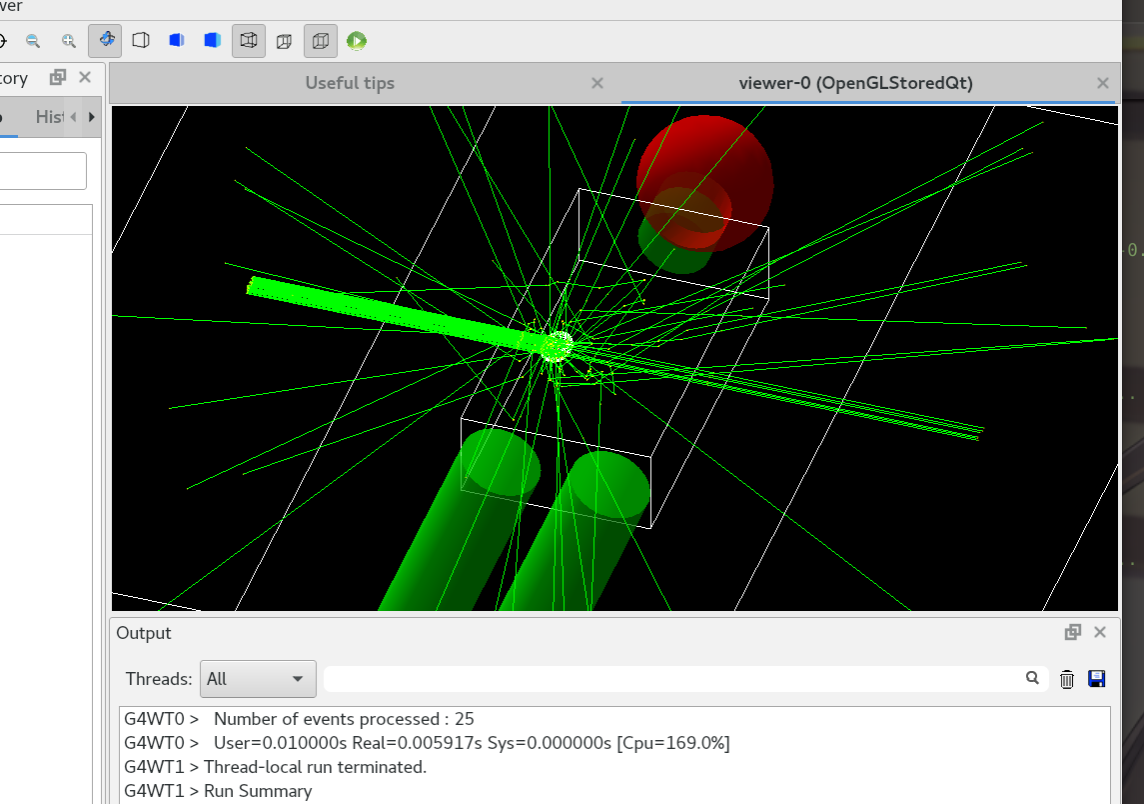
\includegraphics[width=0.5\linewidth]{view.png}
    \caption{可视化界面}
    \label{fig:2}
\end{figure}
在图中可以看到入射的粒子径迹，在身体中发生散射或者反应，继续运动，直到粒子消失或者飞出world。可以看到我们的程序能够正常运行，接下来我们会对存储下来的结果进行展示和分析。
\newpage
\subsection{三维可视化能量沉积}
\begin{figure}[htbp]
    \centering
    \includegraphics[width=0.49\textwidth]{gamma3D.png}
    \includegraphics[width=0.49\textwidth]{proton.png}\\
    \includegraphics[width=0.49\textwidth]{neutron3D.png}
    \caption{(a)光子三维能量沉积 (b)质子三维能量沉积 (c)中子三维能量沉积}
    \label{fig:3}
\end{figure}
图~\ref{fig:3}展示了三种不同入射粒子在三维空间当中的能量沉积，图中每个小方格当中会画出对应空间位置的step在此沉积的能量。可以看到，光子在空间中的能量沉积较为均匀，这是因为光子和身体正常组织与肿瘤组织反应的类型和概率都是相同的，并无特异性，且容易善射，即自由程也较大，所以它的能量分布在各处分布都比较均匀并遍布空间。而对于质子，由于出射的粒子束流是朝向肿瘤方向，且质子反应截面较大，导致自由程较小，故能量沉积主要集中在束流入射的方向。而对于中子来说，在我们定义的反应当中应当为硼中子俘获反应，那由于身体组织和肿瘤组织的硼浓度有差异，所以中子沉积能量在肿瘤区域和身体区域则会产生差异。从上图可以看出我们模型的可靠性。
\newpage
\subsection{对质子的能量沉积求和的分布}
\begin{figure}[htbp]
    \centering
    \includegraphics[width=1.1\linewidth]{penergy.png}
    \caption{质子能量沉积求和的分布}
    \label{fig:4}
\end{figure}
此图展示了我们所模拟的质子能量求和分布，我们对粒子的初始束流能量，束流宽度作了扫描，最后得到了一系列的root文件，并分别绘制了能量沉积分布。我们在其中挑选了几幅具有代表性的分布在此展示，可以看到随着束流能量、宽度的变化，质子能量沉积范围既有比较集中，也有具有长尾的分布。接下来我们将对质子治疗效果进行分析。
\subsection{质子治疗效果评估}
首先我们定义我们治疗效果，通过射线治疗癌症是通过将入射粒子或其反应产物的能量沉积在肿瘤组织当中，从而杀死癌细胞~\cite{WOS:000397979500001}。所以在肿瘤组织当中沉积能量是我们需要考虑的一点，而我们同样需要考虑射线在身体其余正常组织当中沉积的能量，即我们希望在肿瘤组织当中沉积能量要足够高，在身体正常组织当中沉积能量要足够低。我们定义
$$Tissue\_body\_Density\_ratio= E_{tissue}/E_{body} \times \frac{V_{body}}{V_{tissue}}$$
其中$E_{tissue}$和$E_{body}$分别为肿瘤区域和身体区域沉积总能量，$V_{tissue}$和$V_{body}$分别为肿瘤区域和身体区域的总体积。这个值越大，反映出治疗效果越好。

我们绘制了不同的束流宽度下，TissuebodyDensityratio随着粒子入射能量变化的趋势图。
\begin{figure}[htbp]
    \centering
    \includegraphics[width=0.5\linewidth]{pscan.png}
    \caption{TissuebodyDensityratio随着质子入射能量变化的趋势图}
    \label{fig:5}
\end{figure}
从此图我们可以看到，随着束流能量上升，治疗效果先逐渐提升，达到一个最大治疗效果点，再随着能量上升治疗效果逐渐下降，且束流宽度越小，即束流越集中治疗效果越好。总的来说，这和我们已有的知识是符合的，因为质子存在布拉格峰，即当高能质子穿过物质（如人体组织）时，会与原子核和电子相互作用，逐渐损失能量。其能量沉积速率在射程末端急剧上升，形成一个尖锐的峰值（即布拉格峰），之后能量迅速降至零。布拉格峰是和入射能量是由相关的，当入射能量达到特定值时，布拉格峰的位置处于肿瘤区域内，此时能量主要能够沉积在肿瘤区域内，对应图中位置即为能量在80-100MeV左右。
\subsection{对光子的能量沉积求和的分布}
\begin{figure}[htbp]
    \centering
    \includegraphics[width=0.5\linewidth]{gamma.png}
    \caption{光子能量沉积求和的分布}
    \label{fig:6}
\end{figure}
此图展示了我们所模拟的光子能量求和分布，我们同样对粒子的初始束流能量，入射角度作了扫描，最后得到了一系列的root文件，并分别绘制了能量沉积分布。我们在选取了一幅分布图在此展示，可以看到光子能量分布在接近0处有个较高的分布，在其余能量范围分布较为均匀。接下来我们将对光子治疗效果进行分析。
\subsection{光子治疗效果评估}
我们绘制了不同的入射角度下，TissuebodyDensityratio随着粒子入射能量变化的趋势图。
\begin{figure}[htbp]
    \centering
    \includegraphics[width=1\linewidth]{gscan.png}
    \caption{TissuebodyDensityratio随着光子入射能量变化的趋势图}
    \label{fig:7}
\end{figure}

从此图我们可以看到，随着束流能量上升，治疗效果先逐渐提升，接着达到一个平台期，能量再上升时，上升趋势逐渐平缓。且角度正对着肿瘤的时候治疗效果最好。

\subsection{对中子的能量沉积求和的分布}
此图展示了我们所模拟的质子能量求和分布，我们对人体组织的硼浓度，肿瘤组织的硼浓度作了扫描，最后得到了一系列的root文件，并分别绘制了能量沉积分布。
\begin{figure}[htbp]
    \centering
    \includegraphics[width=0.5\linewidth]{neutronE1.png}
    \caption{中子能量沉积求和的分布}
    \label{fig:6}
\end{figure}

我们发现直方图中，事例大多集中在低端，我们为了研究这导致这点的原因，以及我们模拟是否正确，做了以下研究。

首先我们希望知道中子在我们的模拟当中，究竟发生了什么反应，热中子散射，热中子俘获发生了没有。
首先我们将图8以对数坐标绘制。
\begin{figure}[htbp]
    \centering
    \includegraphics[width=0.5\linewidth]{nE1log.jpeg}
    \caption{中子能量沉积求和的分布（对数坐标）}
    \label{fig:7}
\end{figure}
我们能够发现，在沉积能量2.2-2.7GeV范围内，有较多事例。我们注意到热中子俘获的特征沉积能量正是2.79GeV,那么这段能量沉积是否是由热中子俘获导致的呢，我们决定探究一下。

在我们存储的root文件当中，存储了粒子的Particle ID，热中子俘获会产生$^{7}Li$，如果在root文件中找到Particle ID与$^{7}Li$对应的事例，我们则可以验证产生了热中子俘获。于是我们将Particle ID与$^{7}Li$对应的事例的沉积能量绘制出来，得到了对应的能量沉积。如图10所示。
\newpage
\begin{figure}[htbp]
    \centering
    \includegraphics[width=0.5\linewidth]{Li7.jpeg}
    \caption{中子能量沉积求和的分布（对数坐标）（Particle ID与$^{7}Li$对应的事例）}
    \label{fig:8}
\end{figure}
我们看到了这部分事例的存在，且能量范围在中子俘获产生能量对应的区间，对这部分事例，我们检索了其能量沉积的最大值，发现是2.80GeV,这和这和热中子俘获沉积的最大能量也能够对应上，基于此，我们可以认为模拟正确反映了真实发生的物理过程。
\subsection{中子治疗效果评估}
我们绘制了不同的束流宽度下，TissuebodyDensityratio随着人体组织的硼浓度，肿瘤组织的硼浓度变化的趋势图。
\begin{figure}[htbp]
    \centering
    \includegraphics[width=0.5\linewidth]{nscan1.png}
    \caption{TissuebodyDensityratio随着人体组织的硼浓度，肿瘤组织的硼浓度变化的趋势图}
    \label{fig:9}
\end{figure}
从此图我们可以看到，随着肿瘤组织的硼浓度，治疗效果逐渐提升，而在肿瘤组织硼浓度一定、正常组织硼浓度越高时，治疗效果会下降。这也和我们的预期是相符合的。
\newpage
同样的我们还考虑了固定硼浓度，对束流宽度做了扫描。发现束流宽度在一定范围内，治疗效果保持稳定，继续提升宽度则会降低治疗效果。

\begin{figure}[htbp]
    \centering
    \includegraphics[width=0.5\linewidth]{nscan2.png}
    \caption{TissuebodyDensityratio随着束流宽度的变化}
    \label{fig:10}
\end{figure}
总的来说，中子的模拟结果符合我们的预期。
\section{总结}
1.首先在本次作业当中，我们完成了G4代码以及后续分析代码的编写，我们构造了探测器，定义了粒子枪，构建了PhysicsList，在其中定义了具体物理过程，并将模拟结果以root形式存储下来，后续进行分析也验证了我们所使用模型的合理性。

2.我们对三种不同的入射粒子分别进行了分析，并且评估了各自对应的治疗效果，总结了相应的关系：即我们发现
\begin{itemize}
    \item 质子：治疗效果先随着粒子入射能量上升而提升，达到最优，之后下降。束流越集中时治疗效果越好
    \item 光子：治疗效果先随着粒子入射能量上升而提升，接着到达平台期。束流正对肿瘤时治疗效果越好。
    \item 中子：治疗效果先随着肿瘤硼区域浓度上升而提升，且人体组织硼浓度越低时治疗效果越好。且束流宽度在较小时治疗效果能达到最好
\end{itemize}

3.我们对我们模型的正确性进行了检验，深入探索了我们定义的物理过程是否发生，发现我们正确模拟了硼中子俘获的反应的发生，代表了我们所定义的物理过程的合理性、正确性

4.我们也在课堂上进行了汇报，与老师和同学们进行了相关讨论，得到了老师的正面评价。并和其他数个组进行过交流，提供过我们所使用的代码。
\clearpage

\cleardoublepage % 确保参考文献从新页面开始（如果是书籍/报告类文档）
\addcontentsline{toc}{section}{References} % 将“References”添加到目录
\bibliographystyle{unsrt} % 选择参考文献样式（如 plain, unsrt, ieeetr, apalike 等）
\bibliography{ref} % 加载 ref.bib 文件


\newpage

\end{document}
